\section{Information theory quantifiers}\label{sec:quanti}

Dynamical systems are systems that evolve in time.
In practice, one may only be able to measure a scalar time series ${\mathcal X}(t)$ which may be a function of variables ${\mathcal V}=\{ v_1,  v_2,\cdots, v_k\}$ describing the underlying dynamics (i.e. $d{\mathcal V}/dt=f({\mathcal V})$.
Given a time series or other observational data, we try to infer  properties of an unfamiliar system from  the analysis of measured time record of it behavior (time series).  
how much information are these data revealing about the dynamics of the underlying system or processes?
The information content of a system is typically evaluated via a probability distribution function (PDF) $P$ describing the apportionment of some measurable or observable quantity, generally a time series ${\mathcal X}(t)$. 
We can define Information Theory quantifiers as measures able to characterize relevant properties of the PDF associated with these time series, and in this way we should judiciously extract information on the dynamical system under study.
These quantifiers represent metrics on the space of PDFs for data sets, allowing to compare different sets and classifying them according to the properties of underlying processes - broadly, stochastic vs.  deterministic.

In our case, we are interested in chaotic dynamics.
Thus we are interested in metrics which take the temporal both order of observations explicitly into account; i.e. the approach is fundamentally \textit{causal} and \textit{statistical} in nature.
In a purely statistical approach, correlations between successive values from the time series are ignored or simply destroyed via construction of the PDF; while a causal approach focuses on the PDFs of data sequences.

The quantifiers selected are based on symbolic counting and ordinal pattern statistics.
For an application of alternative quantifiers based on Symbolic Dynamics to environmental data, we refer to \cite{Hauhs2008}.
The metrics to be used can be broadly classified along two categories: those which quantify the \textit{information content} of data versus those related to their \textit{complexity}.
Note that we are referring to the space of probability density functions here, not physical space.
For the sake of clarity and simplicity, we only introduce Information Theory quantifiers that are defined on discrete PDFs in this section, since we are only dealing with discrete data (time series).
However, all the quantifiers also have definitions for the continuous case \cite{Shannon1948,Frieden2004} . 

\subsection{Shannon entropy and statistical complexity}

Entropy is a basic quantity that can be regarded to as a measure of the uncertainty associated (information) to the physical process described by $P$.
When dealing with information content, the Shannon entropy is often considered as the foundational and most natural one \cite{Shannon1948,Weaver1949}.
Regarded as a measure of uncertainty, is the most paradigmatic example of these information quantifiers.

Let a $P=\{p_i; i=1,\ldots, N\}$ with $\sum_{i=1}^N p_i = 1$, be a  discrete probability distribution, with $N$ the number of possible states of the system under study.
The Shannon's logarithmic information measure reads
\begin{equation}
\label{Shannon-disc}
{\mathrm S}[P] ~=~ -\sum_{i=1}^{N} p_i \ln \left[ p_i \right] \ .
\end{equation}

If ${\mathrm S}[P] = {\mathrm S}_{\min} = 0$, we are in position to predict with complete certainty which of the possible outcomes $i$, whose probabilities are given by $p_i$, will actually take place. 
Our knowledge of the underlying process described by the probability distribution is maximal in this instance. 
In contrast, our knowledge is minimal for a uniform distribution $P_e = \{ p_i = 1/N, \forall i=1, \ldots , N \}$ since every outcome exhibits the same probability of occurrence, and the uncertainty is maximal, i.e., ${\mathrm S}[P_e] = {\mathrm S}_{\max} = \ln N$.
These two situations are extreme cases, therefore we focus on the `normalized' Shannon entropy, $0 \leq {\mathcal H} \leq 1$, given as
\begin{equation}
\label{shannon-disc-normalizada}
{\mathcal H} [P]~=~{\mathrm S}[P]  / {\mathrm S}_{\max} \ .
\end{equation}

Contrary to information content, there is no universally accepted definition of complexity.
Here, we focus on describing the \textit{complexity of time series} and do not refer to the complexity of the underlying \textit{systems}.
A complex system does not necessarily generate a complex output.
In fact, “simple” models might generate complex data, while “complicated” systems might produce output data of low complexity \cite{Kantz1998}.

An intuitive notion of a quantitative complexity attributes low values both to perfectly ordered data (i.e. with vanishing Shannon entropy) as well as to uncorrelated random data (with maximal Shannon entropy.
For example, the statistical complexity of a simple oscillation or trend (ordered), but also of uncorrelated white noise (unordered) would be classified as low.
Between the two cases of minimal and maximal entropy, data are more difficult to characterize and hence the complexity should be higher.
We seek some functional ${\mathcal C} [P]$ quantifying structures present in the data which deviate from these two cases.
These structures relate to organization, correlational structure, memory, regularity, symmetry, patterns, and other properties \cite{Feldman2008}.
One would like to assume that the degree of correlational structures would be adequately captured by some functional ${\mathcal C} [P]$ in the same way that Shannon's entropy ${\mathrm S}[P]$ \cite{Shannon1948} ``captures" randomness.
Clearly, the ordinal structures present in a process is not quantified by randomness measures, and consequently, measures of statistical or structural complexity are necessary for a better understanding (characterization) of the system dynamics represented by their time series \cite{Crutchfield1998}. 
A suitable measure of complexity can be defined as the product of a measure of information and a measure of
disequilibrium, i.e. some kind of distance from the equiprobable distribution of the accessible states of 
a system. 
In this respect, Rosso and coworkers \cite{Lamberti2004} introduced an effective {\it Statistical Complexity Measure\/} (SCM) ${\mathcal C}$, that is able to detect essential details of the dynamical processes underlying the dataset.
Based on the seminal notion advanced by L\'opez-Ruiz {\it et al.} \cite{LMC1995}, this statistical complexity measure\cite{Martin2003,Lamberti2004} is defined through the functional product form
\begin{equation}
{\mathcal C}[P] ~=~ {\mathcal Q}_{J}[P,P_e] \cdot {\mathcal H}[P]
\label{complexity}
\end{equation}
of the normalized Shannon entropy ${\mathcal H}$, see Eq.~\eqref{shannon-disc-normalizada}, and the disequilibrium ${\mathcal Q}_{J}$ defined in terms of the Jensen-Shannon divergence ${\mathcal J}[ P, P_e]$.
That is,
\begin{equation}
\label{disequilibrium}
{\mathcal Q}_{J} [ P, P_e] ~=~ Q_{0} {\mathcal J}[ P, P_e] ~=~ 
Q_{0} \{ {\mathrm S}[(P + P_e)/2 ] - {\mathrm S}[ P ]/2 - {\mathrm S}[P_e]/2\},
\end{equation}
the above-mentioned Jensen-Shannon divergence and $Q_0$, a normalization constant such that $0 \leq {\mathcal Q}_{J} \leq 1$:
\begin{equation}
Q_0 ~=~ -2 \left\{  {\frac{N+1}{N}}  \ln (N+1) - \ln (2N)  +  \ln N \right\}^{-1} \ ,
\label{q0-jensen-1}
\end{equation}
are equal to the inverse of the maximum possible value of ${\mathcal J} [P,P_e]$.
This value is obtained when one of the components of $P$, say $p_m$, is equal to one and the remaining $p_j$ are zero.

The Jensen-Shannon divergence, which quantifies the difference between probability distributions, is especially useful to compare the symbolic composition between different sequences\cite{JS-Div1991,Grosse2002,JS-Div2014}.
Note that the above introduced SCM depends on two different probability distributions: one associated with the system under analysis, $P$, and the other the uniform distribution, $P_e$.
Furthermore, it was shown that for a given value of ${\mathcal H}$, the range of possible ${\mathcal C}$ values varies between a minimum ${\mathcal C}_{min}$ and a maximum ${\mathcal C}_{max}$, restricting the possible values of the SCM \cite{Martin2006}.
Thus, it is clear that important additional information related to the correlational structure between the components of the physical system is provided by evaluating the statistical complexity measure. 

\subsection{Determination of a probability distribution}

The evaluation of the Information Theory derived quantifiers suppose some prior knowledge about the system; specifically for those previously introduced (Shannon entropy and statistical complexity), a probability distribution associated to the time series under analysis should be provided beforehand. 
The determination of the most adequate PDF is a fundamental problem because the PDF $P$ and the sample space $\Omega$ are inextricably linked. 

Usual methodologies assign to each value of the series ${\mathcal X}(t)$ (or non-overlapped set of consecutive values) a symbol from a finite alphabet $\mathcal{A}=\{a_1,\dots,a_M\}$, thus creating a {\it symbolic sequence} that can be regarded to as a {\it non causal coarse grained\/} description of the time series under consideration. 
As a consequence, order relations and the time scales of the dynamics are completely lost. 

{\it Causal information\/}  may be duly incorporated if information about the past dynamics of the system is included in the symbolic sequence, i.e., symbols of alphabet $\mathcal{A}$ are assigned to a portion of the phase-space or trajectory.
Bandt and Pompe (BP)\cite{Bandt2002} introduced a simple and robust symbolic methodology that takes into account time ordering of the time series by comparing neighboring values in a time series.
The causality property of the PDF allows the quantifiers (based on this PDFs) to discriminate between deterministic and stochastic systems \cite{Rosso2007B}.
The symbolic data are:
{\it (i)\/}~created by ranking the values of the series; and
{\it (ii)\/}~defined by reordering the embedded data in ascending order, which is tantamount to a phase space reconstruction with embedding dimension (pattern length) $D$ and time lag $\tau$.
In this way, it is possible to quantify the diversity of the ordering symbols (patterns) derived from a scalar time series.
Note that the appropriate symbol sequence arises naturally from the time series, and no model-based assumptions 
are needed.
The procedure is the following:
\begin{itemize}
	\item Given a series $\{x_t, \forall \;  t=0, \Delta t, \cdots,N\Delta t \}$, a sequence of vectors of length $D$ is generated.
		\begin{equation}
		(s)\longmapsto\left(x_{t-(d-1)\Delta t},x_{t-(d-2)\Delta t},\dots,x_{t-\Delta t},x_{t}\right) 
		\label{eq:vectores}
		\end{equation}
		Each vector turns out to be the ``history'' of the value $x_t$. Clearly, the longer the length of the vectors $D$, the more information about the history would the vectors have but a higher value of $N$ is required to have an adequate statistics. 
	\item The permutations $\pi=(r_0, r_1, \cdots, r_{D-1})$ of $(0, 1, \cdots, D-1)$ are called ``order of patterns'' of time $t$, defined by:
		\begin{equation}
		\label{eq:permuta}
		x_{t-r_{D-1}\Delta t}\le x_{t-r_{D-2}\Delta t}\le\dots\le x_{t-r_{1}\Delta t}\le x_{t-r_0\Delta t}
		\end{equation}
		In order to obtain an unique result it is considered $r_i<r_{i-1}$ if $x_{t-r_{i}\Delta t}=x_{t-r_{i-1}\Delta t}$.
		In this way, all the $D!$ possible permutations $\pi$ of order $D$, and the PDF $P=\{p(\pi)\}$ is defined as:
		\begin{equation}
		\label{eq:frequ}
		p(\pi)=\frac{\sharp \{s|s\leq N-D+1; (s) \quad \texttt{has type}~\pi\}}{N-D+1}
		\end{equation}
		In the last expression the $\sharp$ symbol denotes cardinality.
\end{itemize}
Thus, an ordinal pattern probability distribution $P = \{ p(\pi_i), i = 1, \dots, D! \}$ is obtained from the time series.
In this way the vector defined by Eq. (\ref{asignation1}) is converted into a unique symbol $\pi$.
We set $r_i < r_{i-1}$ if $x_{s-r_{i}} = x_{s-r_{i-1}}$ for uniqueness.
The only condition for the applicability of the BP method is a very weak stationary assumption: for $k \leq D$, the probability for $x_t < x_{t+k}$ should not depend on $t$.
Regarding the selection of the parameters, Bandt and Pompe suggested working with $4 \leq D \leq 6$ for typical time series lengths, and specifically considered a time lag $\tau = 1$ in their cornerstone paper.

Recently, the permutation entropy was extended to incorporate also amplitude information.
Weighting the probabilities of individual patterns according to their variance alleviates potential issues regarding to ‘high noise, low signal’ patterns, because low-variance patterns that are strongly affected by noise are down-weighted in the resulting ‘weighted ordinal pattern distributions’.
Hence, a potential disadvantage of ordinal pattern statistics, namely the loss of amplitude information, can be addressed by introducing weights in order to obtain a ``weighted permutation entropy (WPE)".
Non-normalized weights are computed for each temporal window for the time series $X$, such that
\begin{equation}
\label{WPE_weigth}
w_j~=~\frac{1}{D}\sum_{k=1}^{D} \left(x_{j+k-1}-\bar{X_j^D}\right)^2.
\end{equation}
In the equation above $x_{j+k-1}-\bar{X_j^D}$ denotes the arithmetic mean of the current embedding vector of length $D$ and its variance $w_j$ is then used to weight the relative frequencies of each ordinal pattern $p_j$.
Originally, this technique was proposed to discriminate patterns immersed in low noise.
We take advantage of the fact that the fixed points are not computed in the WPE.

We computed the normalized permutation Shannon entropy $H$ and the statistical complexity $C$ from these PDFs, and the obtained values are denoted as:
\begin{itemize}
	\item $H_{Val}$, is the normalized Shannon entropy applied to non-causal PDF $P_{Val}$
	\item $H_{BP}$, is the normalized Shannon entropy applied to causal PDF $P_{BP}$
	\item $H_{BPW}$, is the normalized Shannon entropy applied to causal PDF with amplitude contribution $P_{BPW}$
	\item $C_{BP}$, is the normalized statistical complexity applied to non-causal PDF $P_{BP}$
	\item $C_{BPW}$, is the normalized statistical complexity applied to non-causal PDF with amplitude contribution $P_{BPW} $
\end{itemize}

We also used the number of MP as a quantifier\cite{Rosso2012}.
As shown recently by Amig\'o {\it et al.} \cite{Amigo2006,Amigo2007,Amigo2008,Amigo2010}, in the case of deterministic one-dimensional maps, not all the possible ordinal patterns can be effectively materialized into orbits, which in a sense makes these patterns forbidden.
Indeed, the existence of these forbidden ordinal patterns becomes a persistent fact that can be regarded as a new dynamical property.
Thus, for a fixed pattern-length (embedding dimension $D$) the number of forbidden patterns of a time series (unobserved patterns) is independent of the series length $N$.
Remark that this independence does not characterize other properties of the series such as proximity and correlation, which die out with time \cite{Amigo2007,Amigo2010}.

\subsection{Information Planes}

A particularly useful visualization of the quantifiers from Information Theory is their juxtaposition in two-dimensional graphs.
Four information planes are defined:
\begin{enumerate}
	\item Causal entropy vs. non-causal entropy, $H_{BP} - H_{Val}$
	\item Causal entropy with amplitude contributions vs. non-causal entropy, $H_{BPW} - H_{Val}$
	\item Causal complexity vs. causal entropy, $C_{BP} - H_{BP}$
	\item Causal complexity with amplitude contributions vs. causal entropy with amplitude contributions, $C_{BPW} - H_{BPW}$
\end{enumerate}

These diagnostic tools were shown to be particularly efficient to distinguish between the deterministic chaotic and stochastic nature of a time series since the permutation quantifiers have distinct behaviours for different types of processes, see Figs. \ref{fig1} and \ref{fig2}, respectively. 

In the first and second planes a higher value in any of the entropies, $H_{BP}$ and $H_{hist}$, implies an increase in the uniformity of the involved PDF.
The point $(1,1)$ represents the ideal case with uniform histogram and uniform distribution of ordering patterns.
By comparing both planes we can detect falls to fixed points.

In the causality planes $H - C$ not the entire region $0<H_{BP}<1$, $0<C_{BP}<1$ is achievable.
In fact for any PDF the pairs $(H,C)$ of possible values fall between two extreme curves in the plane $H$-$C$ \cite{Anteneodo1996}.
Chaotic maps have intermediate entropy ${\mathcal H}$, while their complexity ${\mathcal C}$ reaches larger values, very close to those of the upper complexity limit \cite{Rosso2007,Olivares2012B}.
For regular processes, entropy and complexity have small values, close to zero. 
Uncorrelated stochastic processes are located in the planar location associated with ${\mathcal H}$ near one and ${\mathcal C}$ near zero.
Ideal random systems having uniform Bandt \& Pompe PDF, are represented by the point $(1,0)$ \cite{Gonzalez2005} and a delta-like PDF corresponds with the point $(0,0)$.

In both information planes (${\mathcal H} \times {\mathcal C}$, see Fig. \ref{fig1} and  ${\mathcal Hval} \times {\mathcal Hbp}$, see Fig. \ref{fig2}), stochastic data are clearly localized at different planar positions than deterministic chaotic ones. 


\begin{figure}
	\centering	
	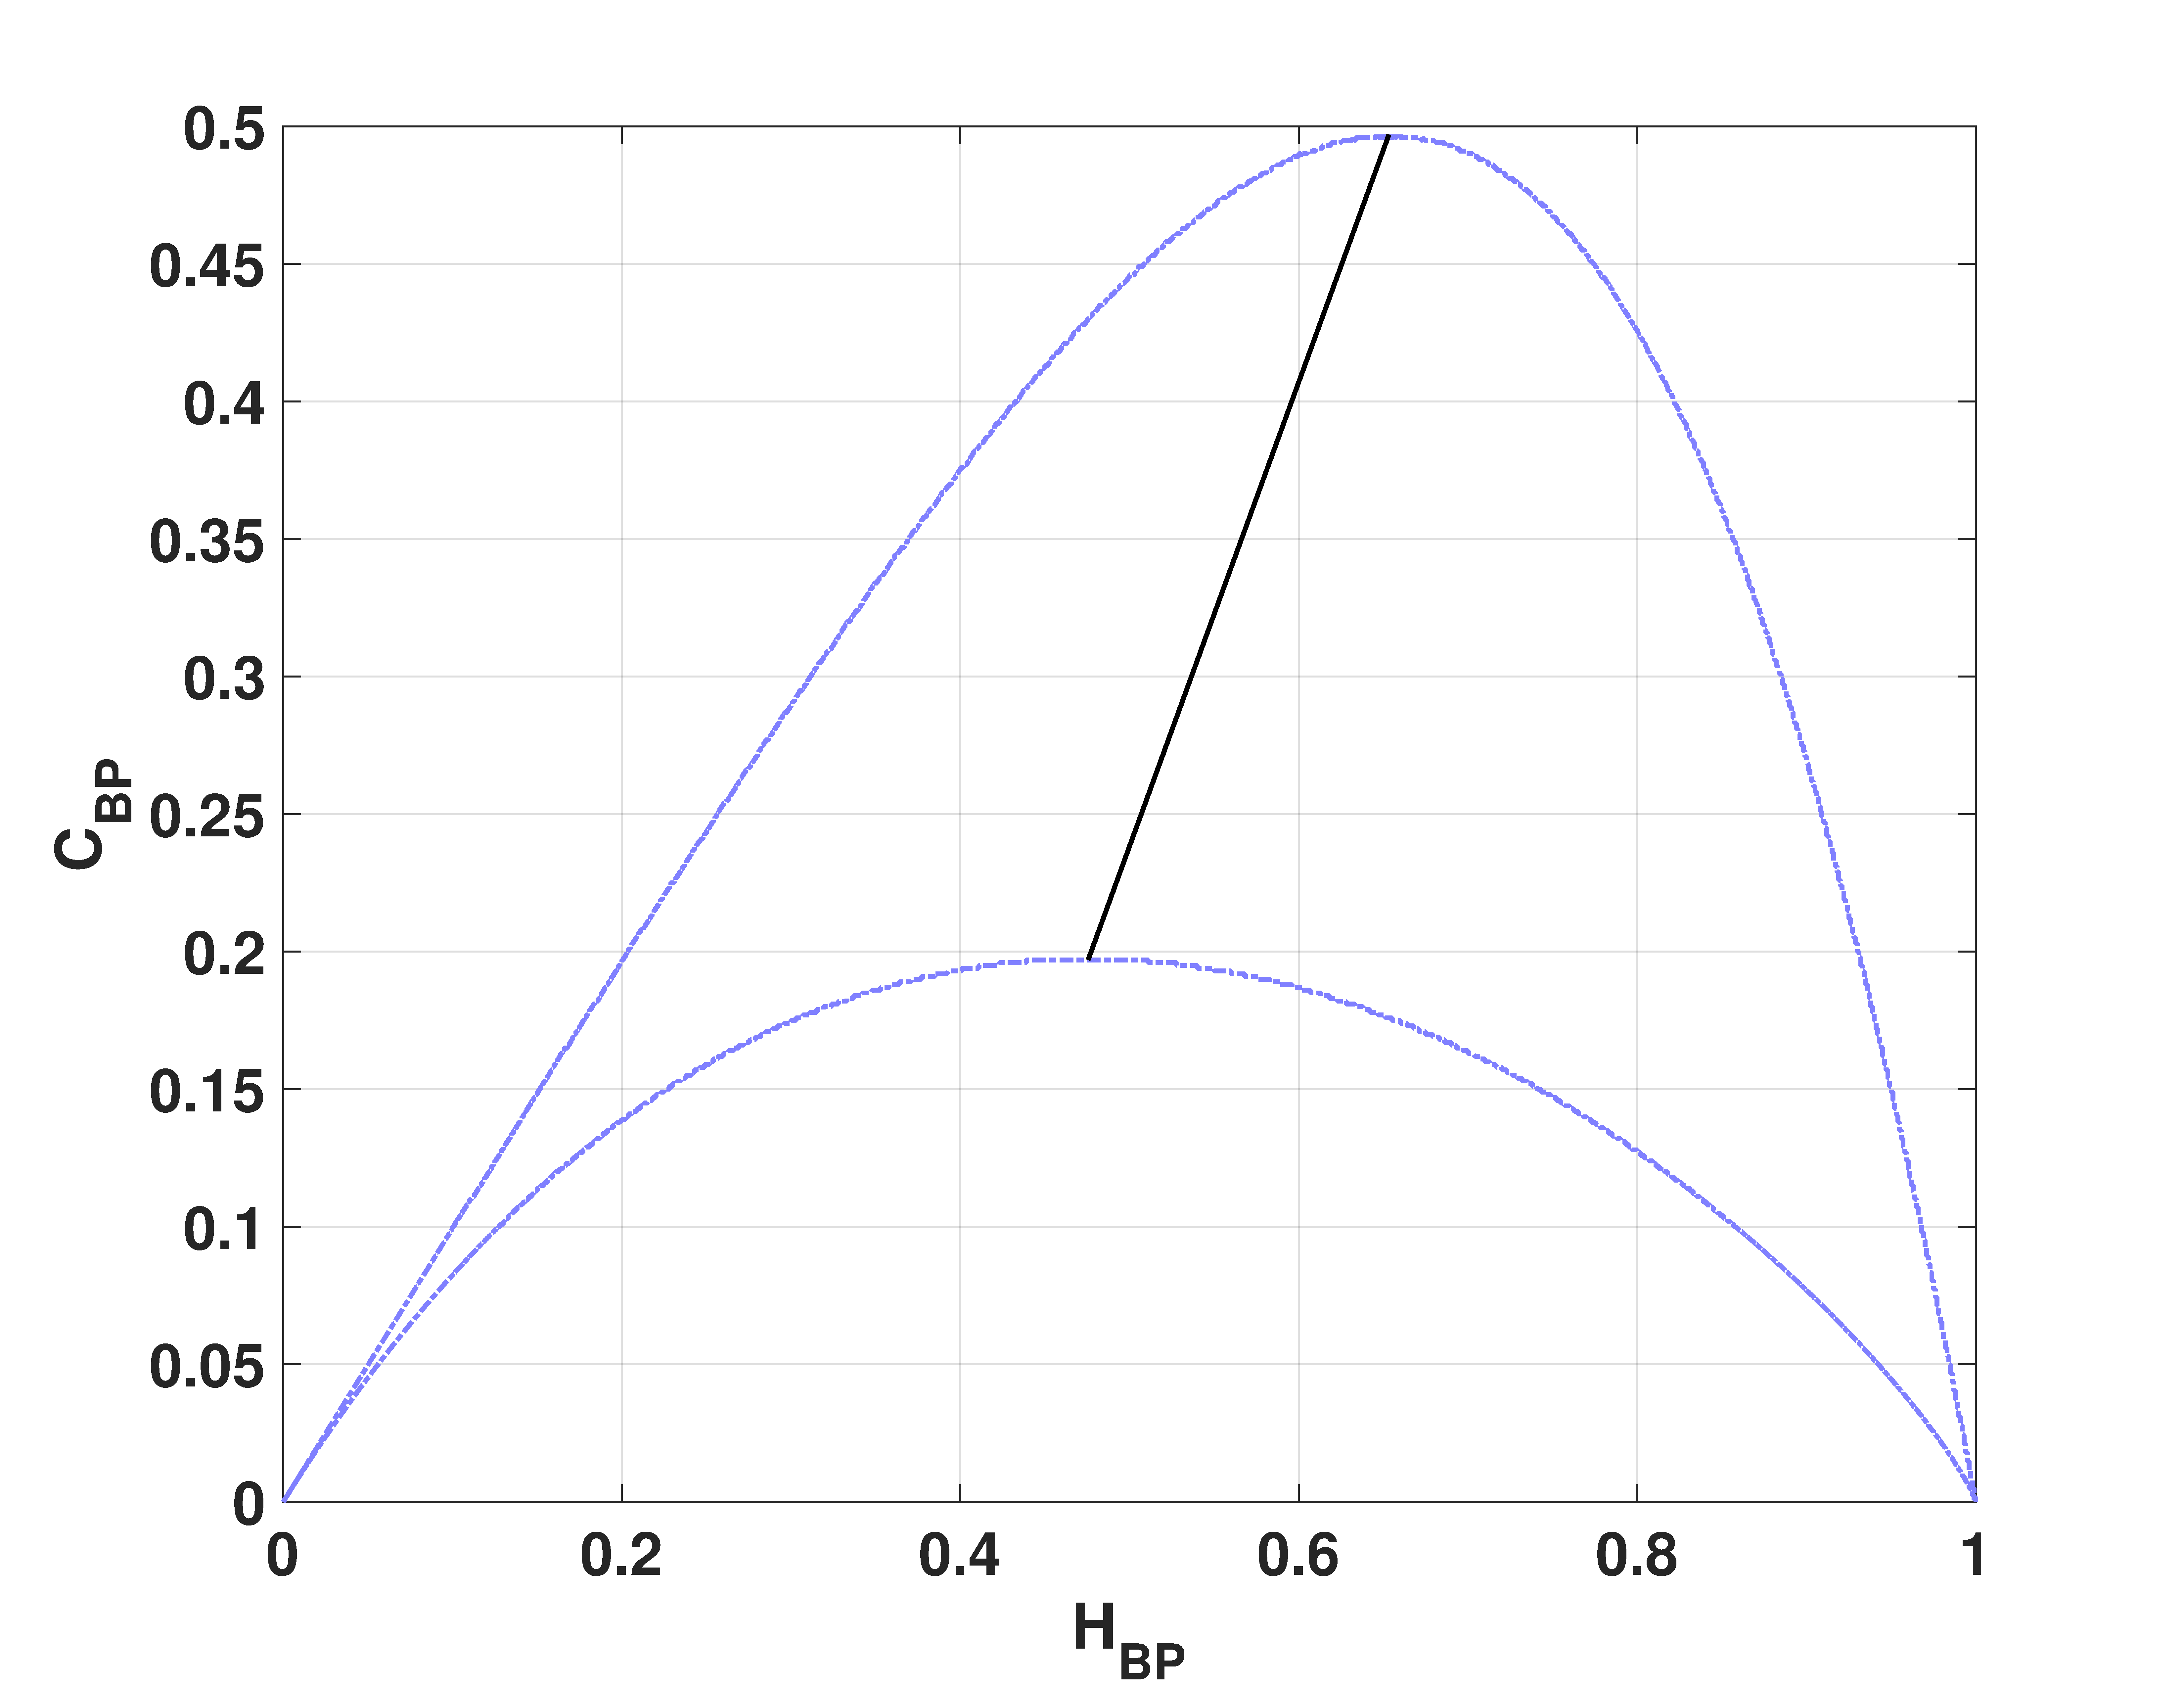
\includegraphics[width= .49\textwidth]{CbpHbp}
	\caption{Entropy-Complexity plane.}
	\label{fig:CbpHbp}
\end{figure}

A full discussion about the convenience of using these quantifiers is out of the scope of this work.
Nevertheless reliable bibliographic sources do exist \cite{Wackerbauer1994,Lopez-Ruiz1995,Rosso2007A,DeMicco2008,Rosso2010,Martin2006,Rosso2012}.


